\newpage % Rozdziały zaczynamy od nowej strony.

\section{Wyniki}
Poniższe dane przedstawione na rysunku \ref{fig:memory} prezentują ilość pamięci RAM wyrażonej w gigabajtach potrzebnej do uruchomienia poszczególnych architektur.
\begin{figure}[H]
    \centering
    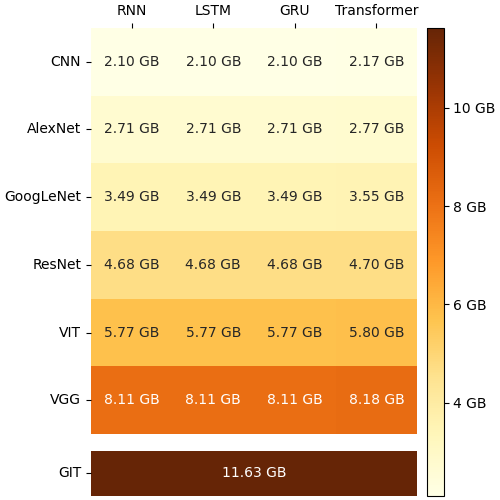
\includegraphics[width=.9\linewidth]{timings/ram}
    \caption{Pamięć RAM potrzebna do uruchomienia testowanych architektur wyrażona w gigabajtach. Opracowanie własne.}
    \label{fig:memory}
\end{figure}
\noindent Można zauważyć, iż największe różnice w ilości potrzebnej pamięci RAM są pomiędzy poszczególnymi modułami kodującymi. W przypadku modułów dekodujących zauważalna różnica jest pomiędzy wykorzystaniem transformera a pozostałymi sieciami rekurencyjnymi. Najpewniej wynika to z tego, iż sieci rekurencyjne przetwarzają tylko jeden element w danym czasie w przeciwieństwie do transformera, który przy pomocy modułu atencji analizuje całą sekwencję w jednym momencie, przez co konieczne jest jej załadowanie do pamięci komputera. Istotnym jest również fakt, iż połowa modułów kodujących potrzebuje ponad 4 GB pamięci, a co za tym idzie, nie było możliwe ich wykorzystanie przy pomocy karty graficznej Nvidia GeForce GTX 1650, ponieważ posiada ona tylko cztery gigabajty pamięci. Tak duża ilość potrzebnej pamięci dotyczy bardzo głębokich sieci oraz wykorzystujących transformer wizyjny. Powodem takiego stanu rzeczy jest fakt, iż w przypadku bardzo głębokich sieci splotowych architektura posiada ogromną liczbę parametrów ze względu na dużą liczbę małych filtrów oraz warstw. Natomiast transformer wizyjny przetwarza obraz do postaci sekwencji, która musi być załadowana w całości, co również znacząco wpływa na rozmiar potrzebnej pamięci.

\subsection{Wydajność uczenia modułów dekodujących}
Dane przedstawione na rysunku \ref{fig:timings-decoders} prezentują czas potrzebny na przetworzenie jednej epoki treningowej poszczególnych kombinacji modułów kodujących oraz dekodujących wykorzystujących wcześniej wytrenowane moduły kodujące.
\begin{figure}[H]
    \centering
    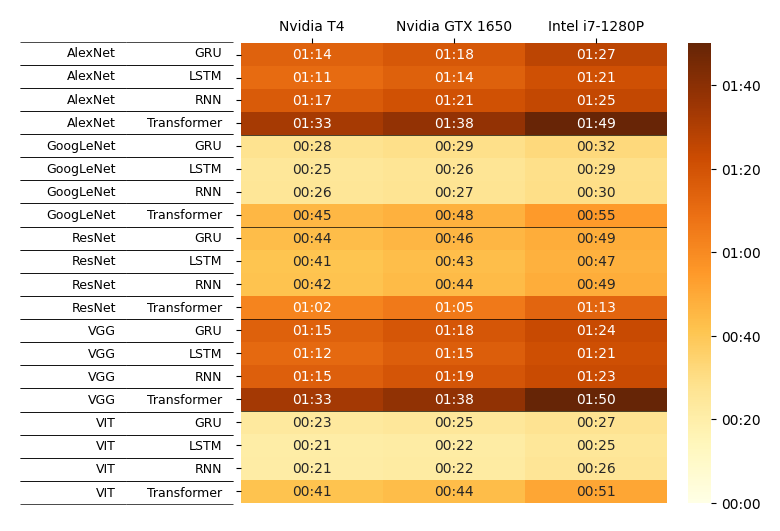
\includegraphics[width=.9\linewidth]{timings/timings_decoders}
    \caption{Czas potrzebny na przetworzenie jednej epoki treningowej poszczególnych kombinacji modułów kodujących oraz dekodujących wykorzystujących wcześniej wytrenowane moduły kodujące. Dane przedstawione w skali logarytmicznej. Opracowanie własne.}
    \label{fig:timings-decoders}
\end{figure}
\noindent Ponownie tak jak w przypadku potrzebnej pamięci do alokacji architektury tutaj również najbardziej zauważalne są różnice czasowe pomiędzy poszczególnymi modułami kodującymi. W przypadku modułów dekodujących różnice są widoczne jedynie pomiędzy wykorzystaniem transformera a pozostałymi sieciami rekurencyjnymi. Co ciekawe, długość przetwarzania nie jest zależna od stopnia skomplikowania sieci. Ze względu na wcześniejsze wygenerowanie danych wejściowych do modułów dekodujących poprzez przetworzenie obrazów przy pomocy wstępnie wyuczonych modułów kodujących, czas potrzebny na przetworzenie jednej epoki treningowej jest zależny od wielkości ostatniej warstwy modułu kodującego, który jest następujący dla poszczególnych sieci:
\begin{itemize}
    \item AlexNet -- 4096,
    \item GoogLeNet -- 1024,
    \item VGGNet -- 4096,
    \item ResNet -- 2048,
    \item VIT -- 768.
\end{itemize}
Biorąc to pod uwagę, łatwo można zauważyć, iż sieć z najmniejszą warstwą końcową, czyli VIT, potrzebuje najmniej czasu na przetworzenie jednej epoki treningowej, a sieci z największą warstwą końcową, czyli AlexNet oraz VGGNet, potrzebuje go najwięcej. W przypadku trenowania również modułu kodującego bez zastosowania wstępnie wyuczonych modeli możliwe byłoby dostosowanie wielkości ostatniej warstwy, w celu zmniejszenia czasu potrzebnego na przetworzenie danych przez moduł dekodujący.
\subsection{Wydajność uczenia modułów kodujących oraz dekodujących}
Dane przedstawione na rysunku \ref{fig:timings-networks} prezentują czas potrzebny na przetworzenie jednej epoki treningowej poszczególnych kombinacji modułów kodujących oraz dekodujących.
\begin{figure}[H]
    \centering
    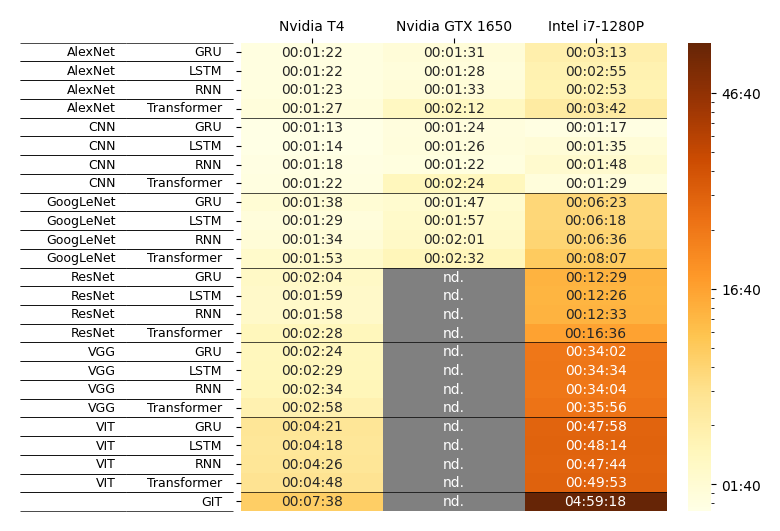
\includegraphics[width=.9\linewidth]{timings/timings_networks}
    \caption{Czas potrzebny na przetworzenie jednej epoki treningowej poszczególnych kombinacji modułów kodujących oraz dekodujących. Opracowanie własne.}
    \label{fig:timings-networks}
\end{figure}
\noindent Niestety ze względu na ograniczenie pamięci RAM karty graficznej Nvidia GTX 1650 nie było możliwe przeprowadzenie treningu sieci zajmujących więcej niż 4 GB pamięci, czyli ResNet, VGG, VIT oraz GIT. W przypadku czasu potrzebnego na przetworzenie danych przy pomocy jednostki CPU rośnie w sposób wykładniczy. Biorąc pod uwagę, iż założeniem przeprowadzonych eksperymentów było przetworzenie zbioru treningowej 500 razy, dla połowy sieci staje się to niewykonalne. Już w przypadku sieci GoogleNet połączonej z jedną z sieci rekurencyjnych, gdzie jedna epoka treningowa zajmuje ponad 6 minut, powtórzenie jej 500 razy zajęłoby 53 godziny. Natomiast w przypadku najdłużej przetwarzającej sieci, czyli GIT, czas ten wyniósłby ponad 100 dni ciągłego przetwarzania. W przypadku pozostałych sieci, gdzie czas kilkudziesięciu godzin jest w wielu momentach akceptowalnym rzędem wielkości, to tak wydłużony czas uczenia znacząco utrudnia reagowanie na wszelkie błędy oraz problemy. Sytuacja jest znacząco lepsza w przypadku wykorzystania jednostki GPU. Pomiędzy modelem dostępnym w wielu komputerach stacjonarnych a modelem dedykowanym do obliczeń na kartach graficznych różnice są stosunkowo niewielkie. W przypadku architektury GIT przetworzenie danych 500 razy zajęłoby około 65 godzin, co w porównaniu do czasu potrzebnego w przypadku wykorzystania jednostki CPU jest osiągalne. Dodatkowo warto wspomnieć, iż korelacja pomiędzy liczbą parametrów ostatniej warstwy modułu kodującego a czasem potrzebny na trening nie pojawia się w tym przypadku. Wynika to z faktu, iż czas trenowania modułu kodującego rośnie o wiele znaczniej wraz z większym skomplikowaniem wykorzystanej architektury.

\subsection{Wydajność generowania podpisów}
Na rysunku \ref{fig:timings-decoders-inference} zostały przedstawione czasy potrzebne na wygenerowanie podpisów obrazków pochodzących z testowego zbioru danych dla poszczególnych architektur.
\begin{figure}[H]
    \centering
    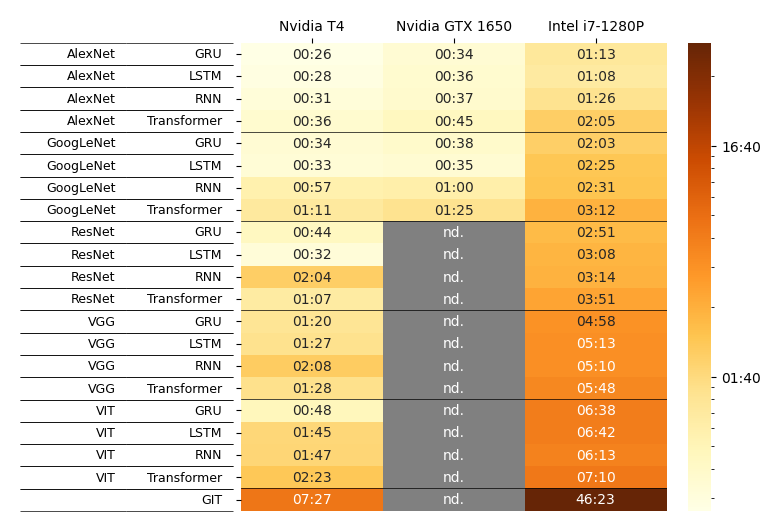
\includegraphics[width=.9\linewidth]{timings/timings_inference_decoders}
    \caption{Czas potrzebny na wygenerowanie podpisów obrazków pochodzących z testowego zbioru danych dla poszczególnych architektur, które zostały wyuczone przy użyciu wcześniej wytrenowanych modułów kodujących. Dane przedstawione w skali logarytmicznej. Opracowanie własne.}
    \label{fig:timings-decoders-inference}
\end{figure}
\noindent W przypadku generowania podpisów konieczne jest wykorzystanie bezpośrednio modułu kodującego, ponieważ w warunkach naturalnych przetwarzane zdjęcie nie jest wcześniej znane. Z tego względu wyniki dla modeli wykorzystujących wcześniej wyuczone moduły kodujące oraz modele trenowane od zera są takie same -- w obu przypadkach obraz przetwarzany jest w ten sam sposób. Wskutek tego nie było możliwe przeprowadzenie eksperymentów przy użyciu karty graficznej Nvidia GTX 1650, tych sieci, których alokacja przekracza 4 GB pamięci. Czas wymagany do przetworzenia zbioru testowego, tak jak w przypadku uczenia architektur, wraz z wykorzystaniem bardziej rozbudowanego modułu kodującego wzrasta, a w przypadku modułów dekodujących znaczące różnice są widoczne jedynie pomiędzy transformerem a pozostałymi sieciami. Ponownie najbardziej wymagającą architekturą okazało się rozwiązanie GIT. Przy jego pomocy przetworzenie tysiąca zdjęć zajęłoby ponad 45 minut, co daje niecałe 3 sekundy na zdjęcie -- taki czas w wielu przypadkach można uznać za akceptowalny, jednakże ponownie pokazuje to, iż prostsze sieci są bardziej przystępne dla osób z ograniczonymi zasobami sprzętowymi. Najszybsza okazała się sieć AlexNet połączona z siecią GRU -- w tym przypadku przetworzenie całego zbioru testowego zajmuje mniej niż pół minuty.

\subsection{Skuteczność otrzymanych rozwiązań}
Wydajność architektur jest niezwykle istotna, ale by móc w pełni ocenić ich przydatność, konieczne jest sprawdzenie skuteczności generowania podpisów. W tym celu wykorzystane zostały metryki BLEU oraz CIDEr. Dane przedstawione na rysunku \ref{fig:metrics} prezentują wartości tychże metryk dla architektury GIT oraz poszczególnych kombinacji modułów kodujących i dekodujących.
\begin{figure}[H]
    \centering
    \begin{subfigure}{.5\textwidth}
        \centering
        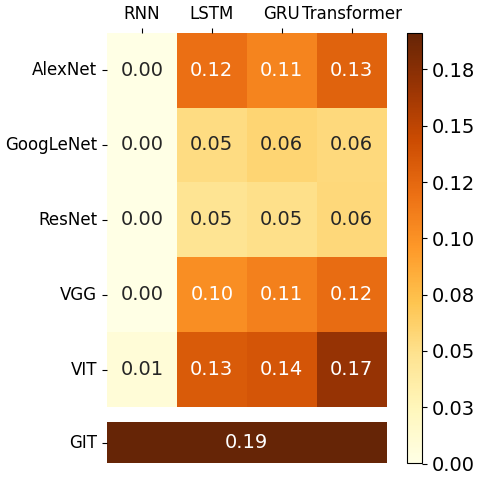
\includegraphics[width=.95\linewidth]{metrics/BLEU}
        \caption{Wartości metryki BLEU}
        \label{fig:bleu}
    \end{subfigure}%
    \centering
    \begin{subfigure}{.5\textwidth}
        \centering
        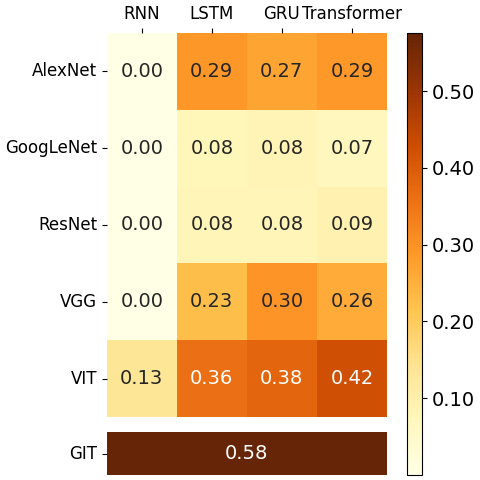
\includegraphics[width=.95\linewidth]{metrics/CIDEr}
        \caption{Wartości metryki CIDEr}
        \label{fig:cider}
    \end{subfigure}%
    \caption{Wartości metryk BLEU oraz CIDEr dla poszczególnych kombinacji modułów kodujących i dekodujących. Opracowanie własne}
    \label{fig:metrics}
\end{figure}
\noindent Wyraźnie widoczna jest bardzo duża skuteczność architektury GIT. W przypadku metryki BLEU jest ona większa jedynie o 0,02 od drugiej najlepszej architektury -- kodera VIT połączonego z transformerem, ale w przypadku metryki CIDEr różnica ta jest już znacznie większa, ponieważ wynosi aż 0,16. Może to świadczyć o lepszej jakości generowanych podpisach.
W przypadku wykorzystywania sieci RNN osiągnięcie sensownych wyników było niemożliwe. W prawie wszystkich przypadkach funkcja straty zbioru walidacyjnego szybko osiągała swoje minimum, zaczynała rosnąć, co najczęściej sygnalizuje przeuczenie modelu -- można to zauważyć na rysunku \ref{fig:training-alexnet-rnn}.
\begin{figure}[H]
    \centering
    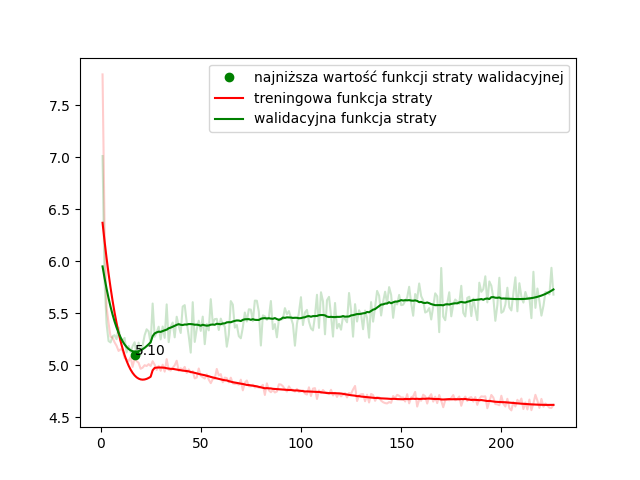
\includegraphics[width=.9\linewidth]{training/alexnet_rnn}
    \caption{Wykres wartości funkcji straty treningowej oraz walidacyjnej dla architektury składającej się z sieci AlexNet i RNN. Opracowanie własne.}
    \label{fig:training-alexnet-rnn}
\end{figure}
\noindent Architektura z wartością funkcji straty na poziomie 5 generowała zdania zawierające jedynie literę „a”, ponieważ jest ona jednym z najczęściej występujących słów w języku angielskim. Wyjątkiem w przypadku wykorzystania sieci RNN jest jej połączenie z transformerem wizyjnym. Dla takiego połączenia metryka BLEU wynosi jedynie 0,01, jednakże wartość CIDEr jest już znacznie wyższa i wynosi 0,13. Wynika to z tego, iż modelowi nie udało się wygenerować pełnych zdań, a jedynie pojedyncze słowa. Przykładowe wyniki zostały przedstawione na rysunku \ref{fig:results-vit-rnn}. Metryka BLEU bierze pod uwagę długość wygenerowanego podpisu, dlatego też w przypadku wygenerowania jedynie pojedynczego słowa, wartość tej metryki jest o wiele niższa w porównaniu do metryki CIDEr.
\begin{figure}[H]
    \centering
    \includegraphics[width=.9\linewidth]{results/vit_rnn}
    \caption{Przykładowe obraz wraz z podpisami wygenerowanymi przez architekturę wykorzystującą transformer wizyjny wraz z siecią RNN. Opracowanie własne.}
    \label{fig:results-vit-rnn}
\end{figure}
\noindent W przypadku tego połączenia funkcja straty walidacyjnej wyniosła wartość 4,5, co można zaobserwować na rysunku \ref{fig:training-vit-rnn}.
\begin{figure}[H]
    \centering
    \includegraphics[width=.9\linewidth]{training/vit_rnn}
    \caption{Wykres wartości funkcji straty treningowej oraz walidacyjnej dla architektury składającej się z transformera wizyjnego i sieci RNN. Opracowanie własne.}
    \label{fig:training-vit-rnn}
\end{figure}
\noindent Jest to stosunkowo lepszy wynik od pozostałych architektur zawierających sieć RNN, biorąc również pod uwagę fakt, iż w przeciwieństwie do pozostałych rozwiązań na wykresie funkcji straty widać dalszy potencjał na malenie jej wartości, a co za tym idzie na nawet lepsze wyniki. Niestety ze względu na ograniczenia czasowe narzucony został limit 500 epok treningowych, które architektura łącząca VIT oraz RNN osiągnęła. Jednocześnie warto zauważyć, że wyuczenie modelu zajęło podobny przedział czasowy, co architektura zawierająca sieć GRU oraz LSTM. W obu tych przypadkach średnia potrzebna na przetworzenie jednej epoki treningowej wyniosła mniej niż 30 sekund, co przy 500 epokach treningowych wynosi około 3 godzin, co jest bardzo zadowalającym czasem. Mimo widocznego potencjału sieci RNN w przypadku połączenia z transformerem wizyjnym nie jest to rozwiązanie, które można uznać za satysfakcjonujące, ponieważ w przypadku wykorzystania sieci RNN w połączeniu z innymi modułami kodującymi, nie udało się osiągnąć zadowalających wyników, a w przypadku wykorzystania transformerów wizyjnych, nie jest to rozwiązanie wydajne ze względu na potrzebę wykorzystania takich samych zasobów komputerowych jak w przypadku wykorzystania sieci GRU lub LSTM. Patrząc na krzywą funkcji straty architektury VIT wraz z siecią GRU widoczne na rysunku \ref{fig:training-vit-gru} można zauważyć jej spłaszczenie w ostatnich epokach treningowych, co nie jest widoczne w przypadku wcześniej omawianego połączenia VIT oraz RNN, jak również w przypadku VIT wraz z klasycznym transformerem, co zostało przedstawione na rysunku \ref{fig:training-vit-transformer}.
\begin{figure}[H]
    \centering
    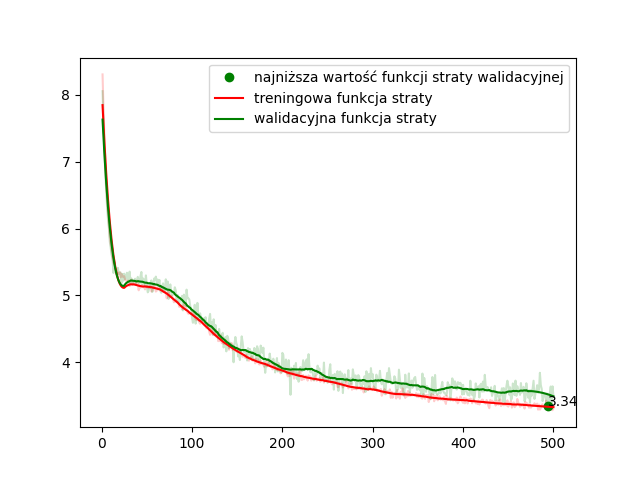
\includegraphics[width=.9\linewidth]{training/vit_gru}
    \caption{Wykres wartości funkcji straty treningowej oraz walidacyjnej dla architektury składającej się z transformera wizyjnego i sieci GRU. Opracowanie własne.}
    \label{fig:training-vit-gru}
\end{figure}
\begin{figure}[H]
    \centering
    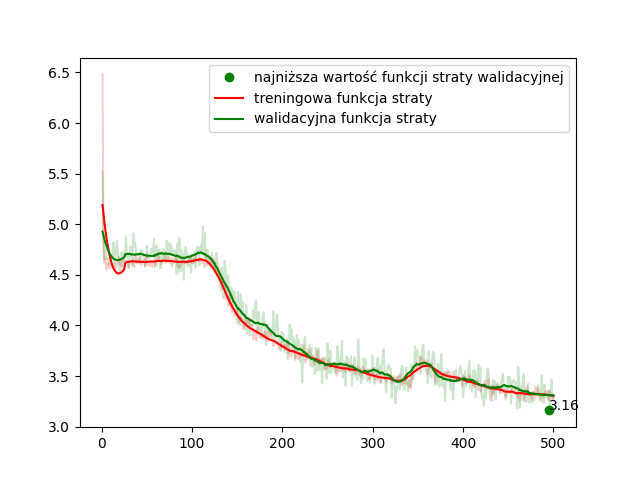
\includegraphics[width=.9\linewidth]{training/vit_transformer_v2}
    \caption{Wykres wartości funkcji straty treningowej oraz walidacyjnej dla architektury składającej się z transformera wizyjnego i klasycznego. Opracowanie własne.}
    \label{fig:training-vit-transformer}
\end{figure}
\noindent Przypadek architektury zawierającej transformer wizyjny i klasyczny jest o wiele bardziej obiecujący niż w przypadku wykorzystania sieci RNN. Wartości funkcji straty są znacznie niższe, widoczna jest dalsza tendencja spadkowa krzywej, a co za tym idzie, możliwe byłoby dalsze poprawianie wyników. Niestety wykorzystywanie klasycznego transformera wiąże się z o wiele większym zapotrzebowaniem zasobów komputerowych. Przetworzenie jednej epoki treningowej architektury VIT i Transformer zajęło średnio 51 sekund, co jest wynikiem prawie dwa razu większym niż w przypadku wykorzystania sieci RNN, GRU lub LSTM. Przykładowe podpisy wygenerowane przez tę architekturę zostały przedstawione na rysunku \ref{fig:results-vit-transformer}.
\begin{figure}[H]
    \centering
    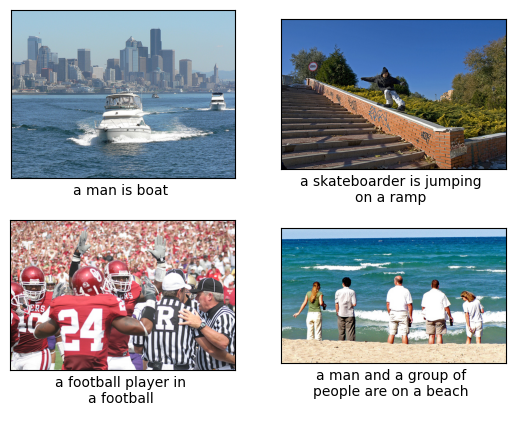
\includegraphics[width=.9\linewidth]{results/vit_transformer}
    \caption{Przykładowe obrazy wraz z podpisami wygenerowanymi przez architekturę wykorzystującą transformer wizyjny wraz z klasycznym transformerem. Opracowanie własne.}
    \label{fig:results-vit-transformer}
\end{figure}
\noindent Można zaobserwować, iż wygenerowane podpisy są o wiele dłuższe niż w porównaniu do architektury VIT i RNN, jednakże brakuje im logicznej spójności. W dużej mierze są one bez sensu, ale zawarte w nich rzeczowniki w większości odnoszą się do faktycznych obiektów znajdujących się na zdjęciach. Jest to dosyć logiczne ze względu na wykorzystanie wstępnie wyuczonych modułów kodujących, które były trenowane na zbiorze danych przeznaczonym do zadań klasyfikacyjnych. Wskazuje to na poprawne rozpoznawanie obiektów znajdujących się na obrazie, jednakże architektura nie potrafi ich połączyć w logiczną całości, za co odpowiedzialny jest moduł dekodujący generujący sekwencję. Mimo wykorzystania zaawansowanego modułu dekodującego, jakim jest transformer, jego danymi wejściowymi cały czas jest pojedynczy wektor reprezentujący obraz. Natomiast podpisy wygenerowane przez sieć GIT, widoczne na rysunku \ref{fig:results-git}, są o wiele bardziej zadowalające, tworzą one zrozumiałe zdania i można zauważyć w nich identyfikacje odpowiednich relacji pomiędzy obiektami znajdującymi się na zdjęciach.
\begin{figure}[H]
    \centering
    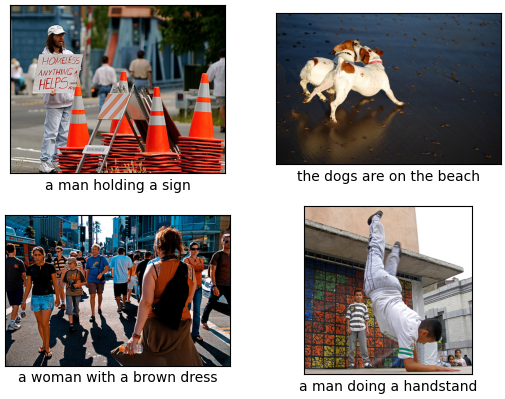
\includegraphics[width=.9\linewidth]{results/git_results}
    \caption{Przykładowe obrazy wraz z podpisami wygenerowanymi przez architekturę GIT. Opracowanie własne.}
    \label{fig:results-git}
\end{figure}
\noindent Tak dobry wynik w porównaniu do pozostałych architektur pokazuje duży wpływ modułu dekodującego na ostateczny rezultat oraz możliwości analizowania obrazu jako całą sekwencję, a nie tylko jako pojedynczy element początkowy. W przypadku tejże sieci warto również przypomnieć, iż w ramach testów wykorzystany został wcześniej wytrenowany model na zbiorze MS COCO, który nie był dostrojony do zbioru Flickr. Niestety tak dobra skuteczność oraz duży potencjał wiążą się z bardzo dużym zapotrzebowaniem na zasoby komputerowe. Wykorzystanie tego rozwiązania zajmuje bardzo dużo czasu i ze względu na ogromną liczbę parametrów nie jest możliwe jego użycie przy pomocy mniejszych kart graficznych, co znacząco wpływa na czas przetwarzania. W przypadku wykorzystania modelu wstępnie wyuczonego takie ograniczenia mogą nie być dużą przeszkodą, ale na pewno korzystając z modelu bez wstępnych wartości parametrów architektury, otrzymanie tak dobrego wyniku może okazać się nieosiągalne ze względu na ograniczenia zasobów komputerowych, czasowych lub budżetowych.

Warto również zwrócić uwagę na wyniki architektury wykorzystującej splotową sieć AlexNet. Rysunek \ref{fig:metrics-transformer} przedstawia wartości metryk wszystkich modułów kodujących w połączeniu z transformerem jako modułem dekodującym. Można na nim zauważyć bardzo dobry wynik w porównaniu do pozostałych architektur.
\begin{figure}[H]
    \centering
    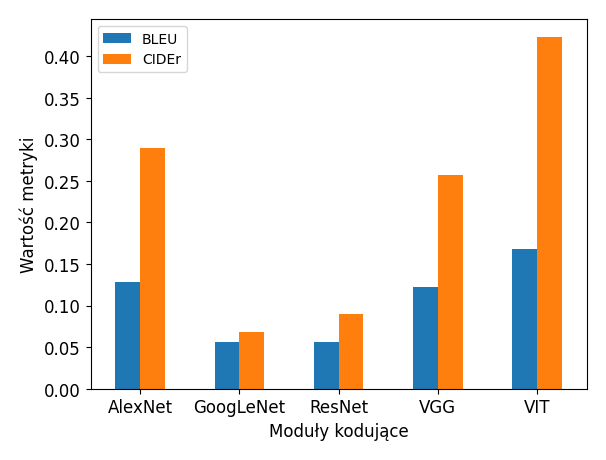
\includegraphics[width=.9\linewidth]{metrics/transformer_metrics}
    \caption{Wartości metryk BLEU oraz CIDEr dla poszczególnych modułów kodujących połączonych z transformerem jako modułem dekodującym. Opracowanie własne.}
    \label{fig:metrics-transformer}
\end{figure}
\noindent Sieć AlexNet ustąpiła jedynie miejsca architekturze GIT oraz kombinacjom modułów wykorzystujących transformer wizyjny. Wynika to z faktu, iż posiadała ona największą ostatnią warstwę w swojej architekturze. Zawierała ona ponad 4 tysiące parametrów -- GoogLeNet, ResNet posiadały ich zdecydowanie mniej, ponieważ odpowiednio: 1024 oraz 2048. Przykładowe podpisy wygenerowane przez architekturę AlexNet wraz z transformerem zostały przedstawione na rysunku \ref{fig:results-alexnet-transformer}. Są one dosyć podobne jakościowo do tych otrzymanych przy pomocy VIT.
\begin{figure}[H]
    \centering
    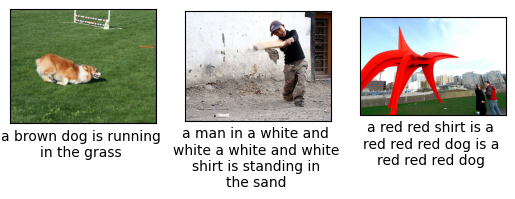
\includegraphics[width=.9\linewidth]{results/alexnet_transformer}
    \caption{Przykładowe obraz wraz z podpisami wygenerowanymi przez architekturę wykorzystującą transformer wizyjny wraz z siecią RNN. Opracowanie własne.}
    \label{fig:results-alexnet-transformer}
\end{figure}
\noindent Zaskakujący jest słabszy wynik architektury VGG, która posiadała taką samą liczbę parametrów jak AlexNet, a mimo wszystko okazała się mniej skuteczna w przypadku obu metryk. Ponownie można zwrócić uwagę na bardzo duży wpływ w analizowaniu obrazu poprzez wykorzystanie transformera wizyjnego, ponieważ pomimo posiadania najmniejszej liczby parametrów -- jedynie 768 -- architektury go wykorzystujące osiągnęły zdecydowanie najlepsze wyniki. Nie można jednocześnie zapomnieć o bardzo dużym wpływie liczby parametrów na czas potrzebny do wyuczenia danych architektur, które można zaobserwować na rysunku \ref{fig:timings-training-decoders-nvidia} dla karty graficznej Nvidia T4.
\begin{figure}[H]
    \centering
    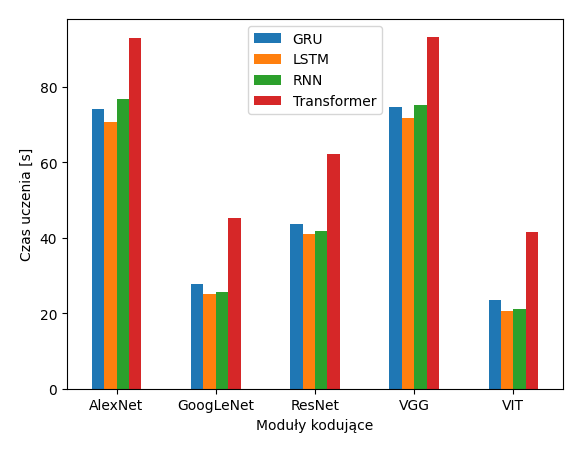
\includegraphics[width=.95\linewidth]{timings/timings_training_decoders_nvidia}
    \caption{Czas przetwarzania jednej epoki treningowej przy użyciu kart graficznej Nvidia T4 dla poszczególnych modułów dekodujących wykorzystujących wstępnie wyuczone moduły kodujące. Opracowanie własne.}
    \label{fig:timings-training-decoders-nvidia}
\end{figure}
\noindent Widoczny jest bezpośredni wpływ liczby parametrów modułów kodujących na czas przetwarzania. Jest to przewidywalnym wynikiem, ponieważ w przypadku większej ilości danych, sieć rekurencyjna musi przetworzyć ich stosunkowo więcej. Interesującym jest fakt, iż nie miało to bezpośredniego przełożenia na lepsze wyniki. Pokazuje to, iż bardzo istotne jest przeanalizowanie obrazu w odpowiedni sposób i najpewniej zwiększenie liczby parametrów w modułach kodujących miałoby w pewnym stopniu wpływ na poprawę skuteczności generowania podpisów, ale porównując różnice w przypadku takich sieci jak GoogLeNet, ResNet, VGG nie są one drastyczne. Warte zweryfikowania na pewno byłoby zwiększenie tejże ilości w przypadku transformera wizyjnego.
% MAYBE może dodać więcej tekstu, żeby lepiej rozłożył się na stronie
\subsection{Porównanie z innymi rozwiązaniami}
Najlepszą z architektur łączących bezpośrednio moduły kodujące i dekodujące okazało się połączenie transformera wizyjnego wraz z klasycznym transformerem. Mimo to wartości metryk otrzymane przy pomocy tego rozwiązania mocno odstają od tych otrzymanych przy pomocy dedykowanych rozwiązań takich jak GIT oraz OFA, co zostało przedstawione w tabeli \ref{tab:comparison}. W przypadku rozwiązania GIT oraz OFA zostały tam umieszczone wyniki podane bezpośrednio przez autorów, jak również te otrzymane przy pomocy udostępnionych bezpośrednio przez autorów wstępnie wyuczonych modeli.
\begin{table}[H]
    \centering
    \caption{Porównanie skuteczności rozwiązania wykorzystującego VIT oraz transformera wizyjnego z innymi rozwiązaniami.}
    \label{tab:comparison}
    \begin{tabular}{|l|l|l|l|l|}
        \hline
        \textbf{Rozwiązanie} & \textbf{BLEU} & \textbf{METEOR} & \textbf{CIDEr} & \textbf{SPICE} \\ \hline
        VIT + Transformer    & 0,17          & 0,18            & 0,42           & 0,10           \\ \hline
        GIT (test)           & 0,19          & 0,17            & 0,58           & 0,13           \\ \hline
        GIT (artykuł)        & 0,40          & 0,30            & 1,31           & 0,23           \\ \hline
        OFA (test)           & 0,33          & 0,28            & 1,03           & 0,21           \\ \hline
        OFA  (artykuł)       & 0,43          & 0,32            & 1,45           & 0,25           \\ \hline
    \end{tabular}
\end{table}
\noindent Wartości metryk otrzymane dla architektury GIT w przypadku BLEU oraz METEOR są nieznacznie wyższe od rozwiązania VIT + Transformer. W przypadku metryk CIDEr i SPICE różnice są bardziej zauważalne, co może świadczyć o lepszej zdolności GIT do zachowania sensu i semantyki w generowanych podpisach. Jednakże porównując wyniki GIT z tymi podanymi bezpośrednio przez autorów architektury, zauważalne są znaczne różnice. Wartości wszystkich metryk dla testowanego wariantu są prawie dwukrotnie mniejsze niż te, które podali autorzy. Takie rozbieżności mogą wskazywać na słabą zdolność architektury do generalizacji na różne zbiory danych lub specyficzne warunki testowe. W przypadku architektury OFA, różnice między wartościami otrzymanymi w badaniach a tymi zawartymi w artykule są niewielkie. Wartości wszystkich metryk podane przez autorów są większe o kilka setnych, co sugeruje, że OFA utrzymuje stabilność wyników i skuteczność w różnych kontekstach. Może to wskazywać na lepszą generalizację i niezawodność architektury OFA w porównaniu do GIT, która również osiągnęła największe wartości w przypadku wszystkich podanych metryk.
